Das Observer Pattern geh�rt zu der Kategorie Verhaltensmuster. 
Mit ihm ist es m�glich �nderungen von einem Objekt an ein anderes Objekt, welches von ersterem strukturell abh�ngig ist, weiterzugeben.
Es ist auch unter dem Namen \textbf{publish-subscribe} bekannt.

\section{Problem}
	Als Beispiel einer Anwendung ohne Observer Pattern betrachten wir folgende Problemstellung:

	\begin{center}
		\fbox{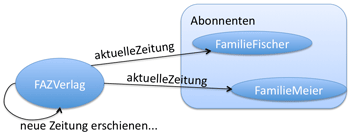
\includegraphics[scale=1]{figure/Observer/einleitungW}} 
			\captionof{figure}{FAZVerlag Problem} 			
		\label{pic:einleitungW}
	\end{center}

	Der FAZ-Verlag versendet die jeweils aktuelle Zeitung an seine Abonnenten, Familie Fischer und Meier.\\
	Bei jeder neuen Zeitung soll eine Auslieferung erfolgen.\\
	
	Nachfolgend ist der Sachverhalt als Klassendiagramm einer simplen L�sung (ohne Observer Pattern) dargestellt:\\

	\enlargethispage{2cm}	

	\begin{center}
		\fbox{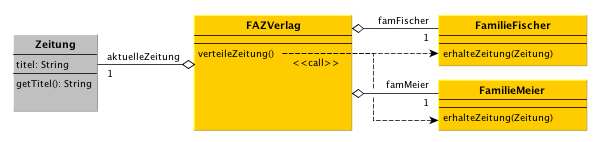
\includegraphics[scale=0.8]{figure/Observer/einleitungI-kl}}
			\captionof{figure}{Klassendiagram FAZVerlag Problem} 			
		\label{pic:einleitungI-kl}
	\end{center}

	Die Familien Fischer und Meier, sowie die Zeitung sind Elemente der Klasse FAZ-Verlag.\\
	Der FAZVerlag ruft einzeln die Funktion erhalteZeitung(Zeitung) auf.\\
	
	\subsection{Eine simple Java Implementierung}
	
		Eine schnelle, sehr unsaubere L�sung ist hier nachfolgend in Java implementiert:\\

		\begin{lstlisting} [caption={Beispiel Java}\label{lst: Smalltalk_bsp},captionpos=b] 
		public class FAZVerlag { 

			private Zeitung aktuelleZeitung; 
			private FamilieFischer famFischer; 
			private FamilieMeier famMeier; 

			//Sobald eine neue Ausgabe existiert
			public void verteileZeitung() { 
			        famFischer.erhalteZeitung(aktuelleZeitung); 
			        famMeier.erhalteZeitung(aktuelleZeitung); 
			} 
		}
		\end{lstlisting}

		Sobald eine neue Ausgabe der Zeitung erscheint, wird f�r jede Familie einzeln deren implementierte Funktion ``erhalteZeitung'' aufgerufen.
		Die Familien sind fest implementiert und k�nnen nicht zur Laufzeit ver�ndert werden.
		

	\subsection{Nachteile}
		\begin{itemize}
			\item{Enge Verbindung zwischen FAZVerlag und Abonnenten}
			\item{Die Erweiterbarkeit ist stark eingeschr�nkt}
			\item{Abonnement bestellen oder abbestellen w�hrend der Laufzeit nicht m�glich.}	
		\end{itemize}


\section{L�sung: Das Observer Pattern}

	F�r eine gute, erweiterbare L�sung: Das \textbf{Observer Pattern}. \\

	"Definiere eine 1-zu-n-Abh�ngigkeit zwischen Objekten, so dass die �nderung des Zustands eines Objekts dazu f�hrt, 
	das alle abh�ngigen Objekte benachrichtigt und automatisch aktualisiert werden." ([GoF], Seite 287) \\
	
	\pagebreak[4]
	
	Der grobe Sachverhalt des Observer Patterns sieht wie folgt aus:
	\begin{center}
		\fbox{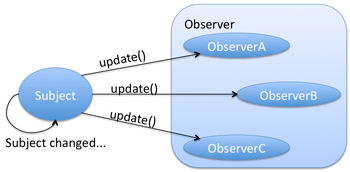
\includegraphics[scale=0.7]{figure/Observer/observer-def-schema}} 
			\captionof{figure}{Observer Pattern Schema} 			
		\label{pic:observer-def-schema}
	\end{center}
	
	Das Observer Pattern besteht aus Objekten (Observer), die sich bei einem anderen Objekt (Subjekt) registrieren.\\
	Sobald sich etwas am Subjekt �ndert, werden die Observer informiert (update). \\

	Hier wird der Aufbau in Form eines Klassendiagramms noch einmal genauer betrachtet:
	\begin{center}
		\fbox{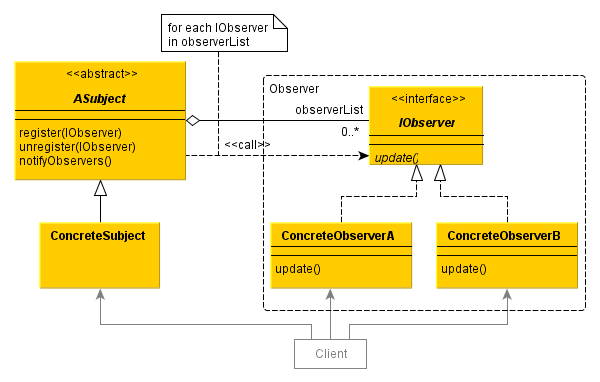
\includegraphics[scale=0.6]{figure/Observer/observer-def-kl}}
			\captionof{figure}{Observer Pattern Klassendiagramm}		
		\label{pic:observer-def-kl}
	\end{center}
	
	Um die Observer an und abzumelden braucht das Subjekt Administrationsmethoden (registrieren, abmelden) und eine Liste der Observer.\\
	Es wird eine Schnittstelle mit mindestens einer Aktualisierungsmethode ben�tigt, um die Observer einheitlich zu informieren.\\
	Von dieser Schnittstelle k�nnen sich dann beliebig viele Objekte ableiten.Jedes dieser Objekte wird durch die selbe Funktion �ber �nderungen informiert.


	\subsection{Variationen}
		Auf Grund des hohen Beliebtheitsgrades des Observer Patterns, haben sich mehrere Variationen gebildet.
		Hier soll nur auf die Varianten der Aktualisierungsmethoden eingegangen werden.\\
	
		Es gibt zwei Varianten von Aktualisierungsmethoden. Das \textbf{Push} und das \textbf{Pull}-Modell.
		
		\subsubsection{Push-Modell}
		
			Das Subjekt �bergibt die Informationen zum Update per Parameter.
		
			\begin{lstlisting}[caption={Beispiel Push-Modell}\label{lst: PushModell_bsp},captionpos=t] 
			public interface IObserver1{ 

			    public void update(int pLength, int pWidth, boolean pVisible, String pName); 
	
			}  
			\end{lstlisting}
		
			\begin{itemize}
				\item[\Checkmark]{ Observer ben�tigt keine Informationen �ber Subjekt -> Starke Entkopplung!}
				\item[\XSolid]{Nicht jeder Observer ben�tigt alle/die selben Parameter!}
				\item[\XSolid]{Bei Erweiterung m�ssen alle Observer angepasst werden\\
					-> Event-Objekt als Parameter anstatt einzelner Parameter\\
					(GUI-Objekte wie Swing nutzen diese Methode)}
			\end{itemize}
		
		\subsubsection{Pull-Modell}
			Das Subjekt verschickt nur eine kleine Benachrichtigung an die Observer. 
			Die Observer m�ssen daraufhin sich selbst die ben�tigten Informationen vom Subjekt holen.
			
			\begin{lstlisting}[caption={Beispiel Pull-Modell}\label{lst: PullModell_bsp},captionpos=t] 
			public interface IObserver2 { 

			    public void update(ConcreteSubject pConcreteSubject); 

			}  
			\end{lstlisting}
			
			\begin{itemize}
				\item[\Checkmark]{Jeder Observer holt sich per Getter nur die ben�tigten Informationen.}
				\item[\Checkmark]{Bei mehreren Subjekten: Eindeutig von welchem Subjekt!}
				\item[\XSolid]{Kann ineffizient werden, da Observer herausfinden muss was sich konkret ver�ndert hat.}
			\end{itemize}

		\enlargethispage{2cm}

		\subsubsection*{Merke:} % kein Eintrag ins Inhaltsverzeichnis mit *
		\begin{itemize}
			\item{Weiss das Subjekt von den Anforderungen der Observer -> Push-Modell}
			\item{Weiss das Subjekt nichts �ber die Observer -> Pull-Modell}
		\end{itemize}

\section{Beispiel}

	Zur�ck zu unserem FAZ-Beispiel.\\
	Durch Anwenden des Observer Patterns entsteht folgendes Klassendiagramm:
	
	\begin{center}
		\fbox{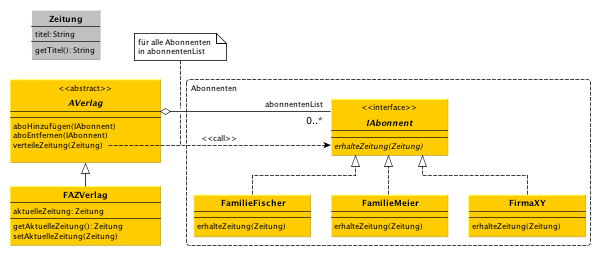
\includegraphics[scale=0.7]{figure/Observer/einleitungV-kl}}
			\captionof{figure}{Observer Pattern FAZVerlag} 		
		\label{pic:einleitungV-kl}
	\end{center}
	
	Der konkrete FAZ-Verlag ist von einer Abstrakten Klassen AVerlag abgeleitet. 
	Jeder Verlag muss einen Abonnenten seiner Liste hinzuf�gen/entfernen und eine Zeitung verteilen k�nnen.
	Alle Abonnenten der Zeitung implementieren das Interface IAbonnent um eine einheitliche Schnittstelle f�r Aktualisierungen zu bieten.

\section{Vor und Nachteile}
	\subsection*{Vorteile} % kein Eintrag ins Inhaltsverzeichnis mit *
	\begin{itemize}
		\item{\textbf{Zustandskonsistenz}: �nderungen werden automatisch an alle Observer weitergegeben.}
		\item{\textbf{Modularit�t}: Es ist m�glich dass mehrere Observer ein Subjekt beobachten, aber auch ein Observer mehere Subjekte.\\
					Die Anzahl der Observer muss zuvor nicht bekannt sein.}
		\item{\textbf{Wiederverwendbarkeit}: Subjekt und Observer sind unabh�ngig variierbar. Beide sind also einzeln wiederverwendbar.}
	\end{itemize}

	\enlargethispage{2cm}	

	\subsection*{Nachteile} % kein Eintrag ins Inhaltsverzeichnis mit *
	\begin{itemize}
		\item{\textbf{Aktualisierungszyklen}: Bei gro�en Systemen kann es zu �nderungsketten kommen, die im schlimmsten Fall rekursive Aufrufe nach sich ziehen (Zyklen). Ebenso k�nnen bei komplexen Systemen einige unn�tige Aktualisierungen auftreten.}
		\item{\textbf{Abmeldung vom Observer}: Es kann schnell passieren, dass man vergisst Observer abzumelden. Speicher wird eventuell nicht freigegeben.}
	\end{itemize}
